\documentclass[12pt, a4paper]{article}
\usepackage[utf8]{inputenc}
\usepackage{CJKutf8}
\usepackage{amsmath}
\usepackage{relsize}
\usepackage{courier}
\usepackage{listings}
\usepackage{enumitem}
\usepackage{titling}
\lstset{basicstyle=\footnotesize\ttfamily,breaklines=true}
\lstset{framextopmargin=50pt,frame=bottomline}
\usepackage{graphicx}
\graphicspath{ {./} }
\bibliographystyle{IEEEtran}


\begin{document}
\begin{titlepage}
    \centering
    \vspace*{\fill}
    {\huge\bfseries CSI4106A Assignment 3 \par}
    \vspace{1cm}
    {\Large Reasoning in Humans and AI \par}
    \vspace{2cm}
    {\Large Group \#1 \par}
    \vspace{0.5 cm}
    {\Large Xiaoxuan Wang (300133594) \par}
    {\Large Victor Li (300146133) \par}
    \vspace{2cm}
    {\large Date: \today \par}
    \vspace*{\fill}
\end{titlepage}


\tableofcontents

\newpage
\section*{Question 1}
\addcontentsline{toc}{section}{\protect\numberline{}Question 1}
\subsection*{e.}
\addcontentsline{toc}{subsection}{\protect\numberline{}e.}
\begin{tabular}{ccc}
1. & $S \rightarrow \lnot Q$ & Premise \\
2. & $P \rightarrow S$ & Premise \\
3. & $\lnot\lnot P$ & Premise \\
4. & $P$ & Double Negation (3) \\
5. & $S$ & Modus Ponens (4, 2) \\
6. & $\lnot Q$ & Modus Ponens (5, 1) \\
\end{tabular}

\subsection*{f.}
\addcontentsline{toc}{subsection}{\protect\numberline{}f.}
\begin{tabular}{ccc}
1. & $T \rightarrow P$ & Premise \\
2. & $Q \rightarrow S$ & Premise \\
3. & $S \rightarrow T$ & Premise \\
4. & $\lnot P$ & Premise\\
5. & $\lnot T$ & Modus Tollens (4, 1) \\
6. & $\lnot S$ & Modus Tollens (5, 3) \\
7. & $\lnot Q$ & Modus Tollens (6, 2) \\
\end{tabular}

\subsection*{g.}
\addcontentsline{toc}{subsection}{\protect\numberline{}g.}
\begin{tabular}{ccc}
1. & $R$ & Premise \\
2. & $P$ & Premise \\
3. & $P \rightarrow (R \rightarrow Q)$ & Premise \\
4. & $R \rightarrow Q$ & Modus Ponens (2, 3) \\
5. & $Q$ & Modus Ponens (1, 4) \\
\end{tabular}

\subsection*{h.}
\addcontentsline{toc}{subsection}{\protect\numberline{}h.}
\begin{tabular}{ccc}
1. & $(R \rightarrow S) \rightarrow Q$ & Premise \\
2. & $\lnot Q$ & Premise \\
3. & $\lnot (R \rightarrow S) \rightarrow V$ & Premise \\
4. & $\lnot (R \rightarrow S)$ & Modus Tollens (2, 1) \\
5. & $V$ & Modus Ponens (4, 3) \\
\end{tabular}

\newpage
\section*{Question 2}
\subsection*{Notation}
$s$ is any student;
$u$ is any university;
$i$ is any individual;
$p$ is any professor;
$c$ is any class.

\addcontentsline{toc}{section}{\protect\numberline{}Question 2}
\subsection*{1.}
\addcontentsline{toc}{subsection}{\protect\numberline{}1.}
$$\forall s(\text{Graduate}(s) \rightarrow \text{UndergraduateDegree}(s))$$

\subsection*{2.}
\addcontentsline{toc}{subsection}{\protect\numberline{}2.}
$$\forall i(\text{UndergraduateDegree}(i) \rightarrow \exists u(\text{Study}(i, u))$$

\subsection*{3.}
\addcontentsline{toc}{subsection}{\protect\numberline{}3.}
Cannot be written as in predicate logic:
``Many'' is not a valid quantifier for predicate logic.

\subsection*{4.}
\addcontentsline{toc}{subsection}{\protect\numberline{}4.}
$$\forall p \exists c(\text{Teach}(p, c) \rightarrow \exists s(\text{Register}(s, c)))$$

\subsection*{5.}
\addcontentsline{toc}{subsection}{\protect\numberline{}5.}
Cannot be written as in predicate logic:
``At least 100'' is not a valid quantifier for predicate logic.

\subsection*{6.}
\addcontentsline{toc}{subsection}{\protect\numberline{}6.}
$$\forall s_1 \forall s_2 \exists c((\text{Register}(s_1, c) \land \text{Register}(s_2, c) \rightarrow \text{Classmate}(s_1, s_2))$$

\subsection*{7.}
\addcontentsline{toc}{subsection}{\protect\numberline{}7.}
Cannot be written as in predicate logic:
``less'' is not a valid quantifier for predicate logic.

\newpage
\section*{Question 3}
\addcontentsline{toc}{section}{\protect\numberline{}Question 3}
\subsection*{Linguistic Variables and Fuzzy Subsets}
\addcontentsline{toc}{subsection}{\protect\numberline{}Linguistic Variables and Fuzzy Subsets}
\subsubsection*{Sleep Quality}
\begin{itemize}
    \item \textbf{Variable Name:} Sleep Quality
    \item \textbf{Range:} 0 to 10 (0 represents very poor sleep quality, and 10 represents excellent sleep quality)
    \item \textbf{Fuzzy Subsets:}
    \begin{enumerate}
        \item \textbf{Poor:} Membership function: Trapezoidal, points (0, 1), (2, 1), (4, 0)
        \item \textbf{Fair:} Membership function: Triangular, points (2, 0), (4, 1), (6, 0)
        \item \textbf{Good:} Membership function: Triangular, points (4, 0), (6, 1), (8, 0)
        \item \textbf{Excellent:} Membership function: Trapezoidal, points (6, 0), (8, 1), (10, 1)
    \end{enumerate}
\end{itemize}
\includegraphics[width=1.1\textwidth]{Figure.3.1.pdf}

\subsubsection*{Leisure Time}
\begin{itemize}
    \item \textbf{Variable Name:} Leisure Time
    \item \textbf{Range:} 0 to 24 hours (including sleeping)
    \item \textbf{Fuzzy Subsets:}
    \begin{enumerate}
        \item \textbf{Minimal:} Membership function: Trapezoidal, points (0, 1), (3, 1), (6, 1), (9, 0)
        \item \textbf{Moderate:} Membership function: Trapezoidal, points (6, 0), (9, 1), (12, 1), (15, 0)
        \item \textbf{Adequate:} Membership function: Trapezoidal, points (12, 0), (15, 1), (18, 1), (21, 0)
        \item \textbf{Plenty:} Membership function: Trapezoidal, points (18, 0), (21, 1), (24, 1)
    \end{enumerate}
\end{itemize}
\includegraphics[width=1.1\textwidth]{Figure.3.2.pdf}

\subsubsection*{Stress Level}
\begin{itemize}
    \item \textbf{Variable Name:} Stress Level
    \item \textbf{Range:} 0 to 15 (0 represents no stress, and 15 represents extremely high stress)
    \item \textbf{Fuzzy Subsets:}
    \begin{enumerate}
        \item \textbf{Calm:} Membership function: Trapezoidal, points (0, 1), (3, 1), (6, 0)
        \item \textbf{Moderate:} Membership function: Triangular, points (3, 0), (6, 1), (9, 0)
        \item \textbf{Intense:} Membership function: Triangular, points (6, 0), (9, 1), (12, 0)
        \item \textbf{Extreme:} Membership function: Trapezoidal, points (9, 0), (12, 1), (15, 1)
    \end{enumerate}
\end{itemize}
\includegraphics[width=1.1\textwidth]{Figure.3.3.pdf}

\subsection*{Fuzzy Rules}
\addcontentsline{toc}{subsection}{\protect\numberline{}Fuzzy Rules}
\begin{enumerate}
    \item IF Stress is \textbf{Intense} and Leisure is \textbf{Minimal} THEN Sleep Quality is \textbf{Poor}.
    \item IF Stress is \textbf{Calm} or \textbf{Moderate} and Leisure is \textbf{Moderate} THEN Sleep Quality is \textbf{Fair}.
    \item IF Stress is \textbf{Extreme} or Leisure is \textbf{Plenty} THEN Sleep Quality is \textbf{Excellent}.
\end{enumerate}

\subsection*{Fuzzy Inference Example}
\addcontentsline{toc}{subsection}{\protect\numberline{}Fuzzy Inference Example}
\subsubsection*{Define Input}
\begin{itemize}
    \item \textbf{Stress Level:} 10
    \item \textbf{Leisure Time:} 10 hours
\end{itemize}

\subsubsection*{Fuzzify}
\begin{itemize}
    \item \textbf{Stress Level (10):} Intense = $\frac{2}{3}$, Extreme = $\frac{1}{3}$
    \item \textbf{Leisure Time (10 hours):} Moderate = 1
\end{itemize}

\subsubsection*{Apply Fuzzy Rules}
\begin{enumerate}
    \item \textbf{Rule 1:} IF Stress is Intense ($\frac{2}{3}$) and Leisure is Minimal (0) THEN Sleep Quality is Poor (0).
    \item \textbf{Rule 2:} IF Stress is Calm (0) or Moderate (0) and Leisure is Moderate (1) THEN Sleep Quality is Fair (0).
    \item \textbf{Rule 3:} IF Stress is Extreme ($\frac{1}{3}$) or Leisure is Plenty (0) THEN Sleep Quality is Excellent ($\frac{1}{3}$).
\end{enumerate}

\subsubsection*{Defuzzify}
\begin{itemize}
    \item Aggregate the fuzzy outputs:
    \begin{itemize}
        \item \textbf{Poor:} 0
        \item \textbf{Fair:} 0
        \item \textbf{Good:} 0
        \item \textbf{Excellent:} $\frac{1}{3}$
    \end{itemize}
    \item Fuzzy subset ``Excellent" is the maxima.
    \item Average of the maxima is $\frac{6 + 10}{2} = 8$

\end{itemize}

Based on the given inputs, the calculated sleep quality is 8, which is excellent.

\newpage
\section*{Question 4}
\addcontentsline{toc}{section}{\protect\numberline{}Question 4}
\subsection*{Constraint-Based Reasoning}
\addcontentsline{toc}{subsection}{\protect\numberline{}Constraint-Based Reasoning}
\subsubsection*{Question}
Source: \cite{Bhatia_2023a}

The percentage of marks obtained by seven girls G1, G2, G3, G4, G5, G6 and G7 in a class are compared. All the girls have obtained different percentages of marks. G4 has the lowest percentage. G3 has a higher percentage than G5, but less than G1. The percentage of G6 is less than G2. G7 has the highest percentage. G1 has a percentage greater than only three girls.

Who has the third lowest percentage?

\begin{enumerate}[label=(\Alph*)]
    \item G1
    \item G4
    \item G3
    \item G7
\end{enumerate}

\subsubsection*{Analysis}
This question showed several constraints on the mark of each girl, and each of the mark has been limited by at least one constraint. Therefore, the question is a constraint-based reasoning question.

There is no other type of reasoning intertwined.

To solve the question, since G1's mark is greater than only three girls, and G4 is the lowest, G1 and G4 are excluded and G1 has the 4th lowest mark. G3 has higher mark than G5 but lower than G1, indicating that G3 has either second lowest or third lowest mark. G7 has the highest mark means G7 is excluded, too. Therefore, the only possible answer left is G3, which is C.

The problem-specific information involves the unique constraints given about each girl's percentage relative to others, such as G4 having the lowest percentage, G3 having a higher percentage than G5 but less than G1, G6 having a percentage less than G2, and G7 having the highest percentage. The generic aspect of constraint-based reasoning in this problem lies in the logical deductions that can be made based on the given constraints. The solver must use deductive reasoning to establish relationships between the percentages of different girls, considering the given information about their relative positions.


\subsection*{Inductive Reasoning}
\addcontentsline{toc}{subsection}{\protect\numberline{}Inductive Reasoning}
\subsubsection*{Question}
Source: \cite{Bhatia_2023b}

In a certain code, the word COMPAQ is written as DQNRBS and SONY is written as TQOA. In the same code, how is MOTOROLA written?

\begin{enumerate}[label=(\Alph*)]
    \item NPUPSPMB
    \item INUNSNMB
    \item NQUQSQMC
    \item OPUPUPIB
\end{enumerate}

\subsubsection*{Analysis}
In this question, we need to find the relationship between two plaintexts and two ciphertexts, then we need to apply the rule to a new plaintext ``MOTOROLA". The question involves identifying a pattern or rule based on the provided examples and then applying that rule to a new case, which makes a good example of inductive reasoning problem.

This question also involves commonsense reasoning, since we need to know the sequence of alphabet to find the hidden rule.

To solve this problem, we can observe that each letter at odd position has shifted backwards by 1, while each letter at even position has shifted backwards by 2. (e.g. C $\rightarrow$ D, O $\rightarrow$ Q). Then, the word ``MOTOROLA" should be written as ``NQUQSQMC". Therefore, the answer should be C.

The specific rule used in this problem is the replacement of each letter by the letter that appears two positions later in the English alphabet and the arrangement of letters in the original words (COMPAQ, SONY) are specific to this problem. The concept of identifying a pattern or rule in a given set of examples, the idea of applying the identified rule to a new case (inductive reasoning), and the use of alphabetical positions and relationships are transferable to various problems.


\subsection*{Analogical Reasoning}
\addcontentsline{toc}{subsection}{\protect\numberline{}Analogical Reasoning}
\subsubsection*{Question}
Source: \cite{Gajanand_2022b}

Directions: In each of the following questions, select the related word from the given alternatives: Botany : Plants :: Entomology : ?

\begin{enumerate}[label=(\Alph*)]
    \item Insects
    \item Snakes
    \item Birds
    \item Plants
\end{enumerate}

\subsubsection*{Analysis}
The given question is a typical example of inductive reasoning, asking to select the related word based on the example answer. The example tells the relation between word ``Botany" and word ``Plants", which implies that Botany is the study of plants. Then, the question gives a new word Entomology and asks the test-taker for the corresponding subject.

Commonsense reasoning about biological subjects is intertwined.

Since the Entomology is the study of insects, the answer is A.

The problem-specific elements are the specific terms involved (Botany, Plants, Entomology, Insects). The relationship of (field, studied object) is transferable to other fields. For instance, if the analogy were Zoology : Animals :: Ornithology : ?, one could apply the same logic to find that the answer is likely to be a specific type of animal studied in ornithology (birds).

\subsection*{Temporal Reasoning}
\addcontentsline{toc}{subsection}{\protect\numberline{}Temporal Reasoning}
Source: \cite{Singh_2020}

\subsubsection*{Question}
If it was Friday on 3rd date of a month, then which day would come on the 4th day after 21st date of that month?

\begin{enumerate}[label=(\Alph*)]
    \item Tuesday
    \item Monday
    \item Thursday
    \item Saturday
\end{enumerate}

\subsubsection*{Analysis}
The question involves reasoning about the days of the week based on specific dates, demonstrating temporal reasoning. It requires understanding the sequential progression of days within a month, which is a temporal concept.

The question involves counting days, which requires basic mathematical reasoning.

To address this issue, it's essential to take into account the chronological order, the time span, and utilize the day of the week to specify the particular time.

The 4th day after 21st date of that month is 25th. Given the 3rd date of a month was Friday, we can calculate to know the 24th is also a Friday ($3 + 7 \times 3 = 24$). Therefore, the 25th should be Saturday, which is D.

The specific days and dates mentioned are problem-specific. Knowing the day on the 3rd date and calculating the day four days after the 21st date applies only to this problem. Understanding the concept of days, weeks, and dates, the ability to count days, and understand the cyclic nature of days in a week are transferable to similar problems.

\subsection*{Spatial Reasoning}
\addcontentsline{toc}{subsection}{\protect\numberline{}Spatial Reasoning}
\subsubsection*{Question}
Source: \cite{Gajanand_2022a}

Which number is on the face opposite to 6?

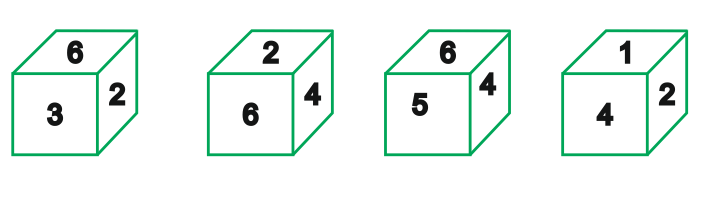
\includegraphics[width=1\textwidth]{Figure.4.5.png}

\begin{enumerate}[label=(\Alph*)]
    \item 4
    \item 3
    \item 2
    \item 1
\end{enumerate}

\subsubsection*{Analysis}
In this question, we need to imagine a cube with numbered sides and rotate it in our head to get the answer. It requires the ability to mentally manipulate the cube in three dimensions, making the problem a good example of a spatial reasoning problem.

While the primary focus is on spatial reasoning, there may be elements of logical reasoning involved as well. For instance, one might need to apply deductive reasoning to eliminate certain options based on the spatial configuration of the cube. Additionally, numerical reasoning could play a role in identifying patterns or relationships between the numbers on different faces.

To solve this problem, we can start with number 6. Based on the first 3 graphs of the cube, we know that number 2, 3, 4 and 5 are the neighbors of number 6, leaving 1 the only option being opposite to 6. Therefore, the answer is D.

Each number on each side of the cube is problem-specific. The ability to mentally construct and manipulate a 3D object is general and transferable to other spatial reasoning problem.

\newpage
\section*{Question 5}
\addcontentsline{toc}{section}{\protect\numberline{}Question 5}

\subsection*{Glittering Generality}
\addcontentsline{toc}{subsection}{\protect\numberline{}Glittering Generality}

\includegraphics[width=0.6\textwidth]{Figure.5.1.png}
Source: \cite{Jordan}

This poster embodies Obama's presidential campaign, portraying him as a symbol of hope. It bears a striking resemblance to the Che Guevara poster, symbolizing the revolutionary spirit of the younger generations who rallied behind Obama's campaign. In this poster, the word “hope” is positive, but it is very abstract, and the word ``hope" is not true or false. The poster implies that Obama will bring hope to the U.S., but people do not know if Obama will be able to bring Hope. Che Guevara is one of the most famous persons in the 20th century. He made great contributions to Cuba. The style of the poster with the word “hope” implies Obama is the Che Guevara of the U.S.


\subsection*{Card Stacking}
\addcontentsline{toc}{subsection}{\protect\numberline{}Card Stacking}

\includegraphics[width=1\textwidth]{Figure.5.2.png}
Source: \cite{Roots_Corporation_2023}

Roots is a well-known Canadian clothing brand that typically runs promotional events around Black Friday. In the picture above, the phrase ``Extra 30\% off sale" is prominently placed in the center with the largest font. However, on the left side of the image, there is a disclaimer with the smallest font stating ``Some exclusions and conditions apply" with an accompanying link. The link explains details on restrictions for the ``Additional 30\% off sale," including conditions like ``Receive an additional 30\% off select sale styles as marked and reflected at checkout on roots.com and in-store" and ``Offer cannot be combined with any other coupons, discounts, offers or promotions"…
By minimizing the negative aspects in smaller font, the seller is trying to entice consumers to browse their products. When consumers find clothing that they prefer and consider purchasing, even if those items are not within the discounts, they may still consider making the purchase. This strategy subtly guides consumers towards exploring the brand's offerings.


\subsection*{Loaded Questions}
\addcontentsline{toc}{subsection}{\protect\numberline{}Loaded Questions}

\includegraphics[width=1\textwidth]{Figure.5.3.png}
Source: \cite{NBA_2012}

In 2012, Radio host Jim Rome asked David Stern who is the NBA commissioner if the league rigged the lottery for the league-owned Hornets. After Stern said that question is ``ridiculous", he asked Rome as a respond: ``Have you stopped beating your wife yet?".
This question is very tricky because it is based on a statement ``Have you ever hit your wife?" If Rome answered ``yes", it will indirectly admit to ``I have beaten my wife before"; but if answered ``no", the situation will become much more serious. If a question is based on an unverified statement, there is no necessity to answer that question. Therefore, the correct response for Rome should be to directly refute the assumed statement by Stern, ``I have never hit my wife," rather than answering yes or no.

\subsection*{Unrelated Testimonial}
\addcontentsline{toc}{subsection}{\protect\numberline{}Unrelated Testimonial}

\includegraphics[width=1\textwidth]{Figure.5.4.png}
Source: \cite{Kiefer_2023}

Beats headphones gained popularity in a decade ago, originally designed to meet the demand among teenagers for stylish headphones. The intention behind the headphone's design was to cater to the aesthetic preferences of young individuals. Consequently, Beats sought the endorsement of basketball star LeBron James and soccer sensation Erling Haaland to promote their products. Although Beats headphones are not specifically designed for sports, James and Haaland are both popular sports figures among teenagers. Therefore, Beats selected them as brand ambassadors to enhance the popularity of their headphones among the younger demographic.

\subsection*{Name Calling}
\addcontentsline{toc}{subsection}{\protect\numberline{}Name Calling}
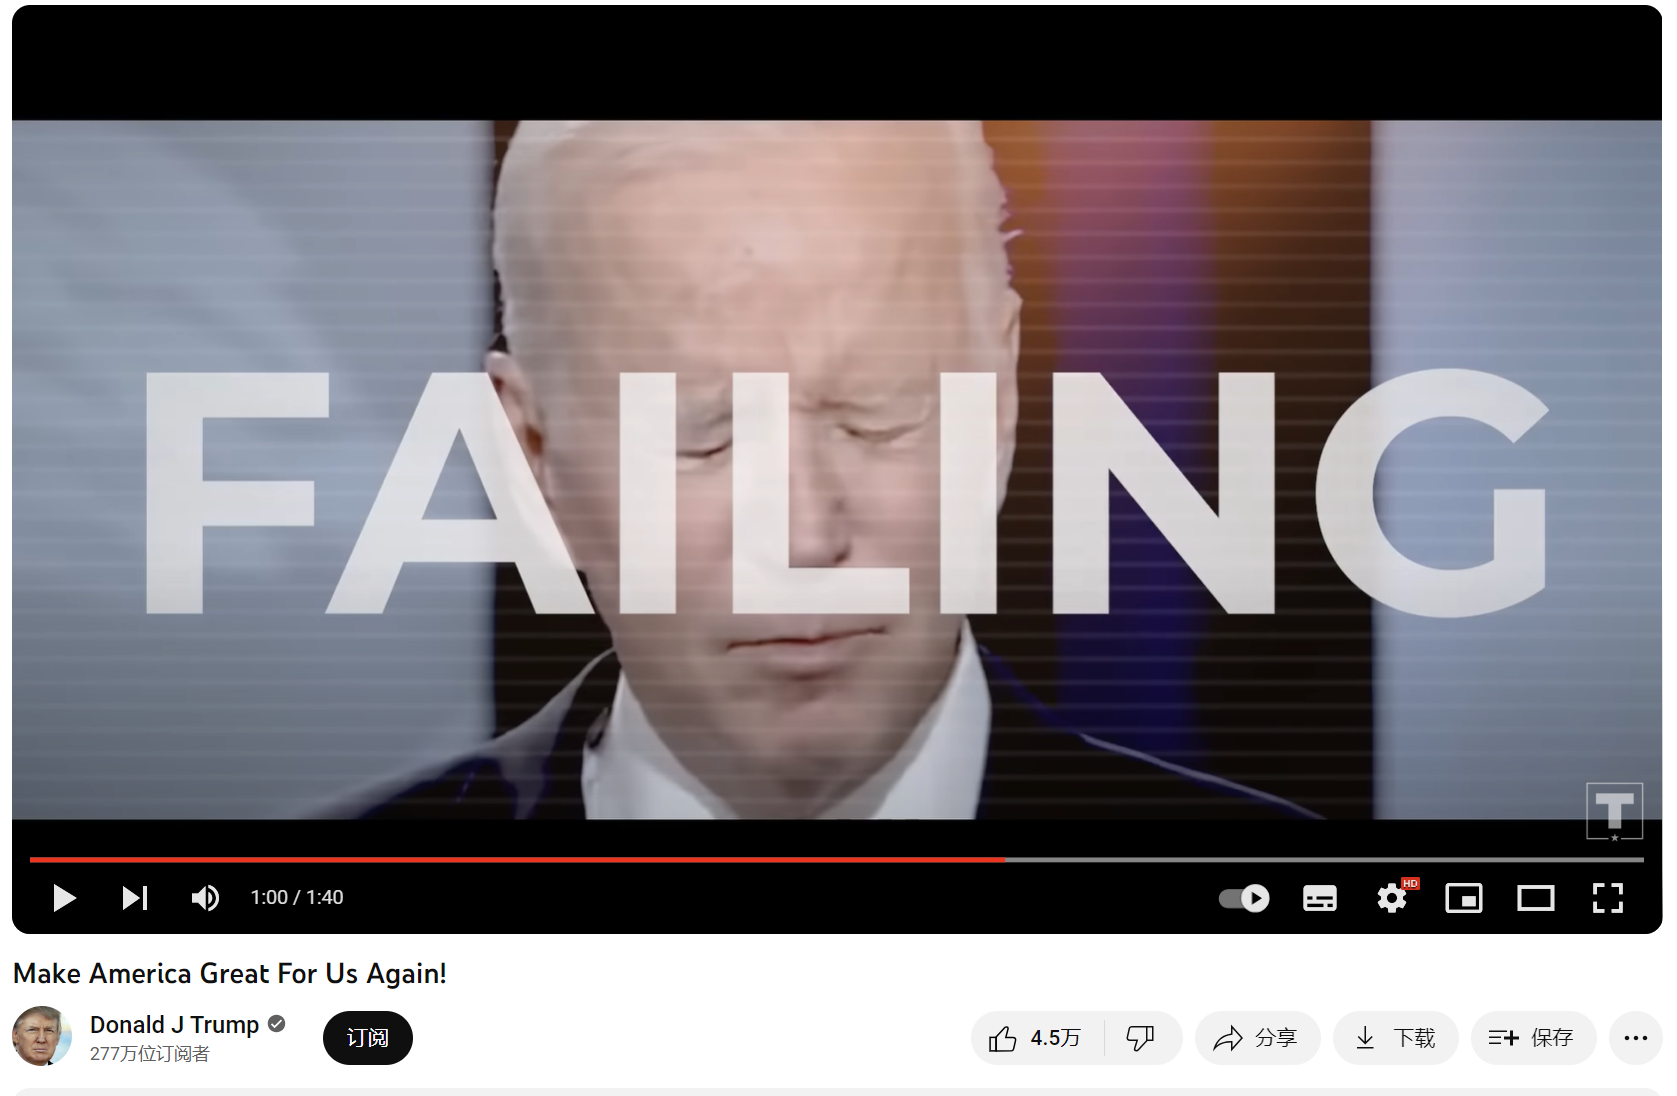
\includegraphics[width=1\textwidth]{Figure.5.5.png}
Source: \cite{MAGA_2023}

This is a political campaign video of Donald J Trump in 2023. In this video, it lists a lot of social, economic, and political problems that the U.S. is facing, and it also mentions. Then the video tags Joe Biden as a failing and weak president. The video attacks that Joe Biden cannot lead the U.S. and Donald Trump can do better than him.

\newpage
\section*{Question 6}
\addcontentsline{toc}{section}{\protect\numberline{}Question 6}
\includegraphics[width=1\textwidth]{Figure.6.pdf}

\newpage
\section*{Question 7}
\addcontentsline{toc}{section}{\protect\numberline{}Question 7}
\subsection*{Mathematical Reasoning}
\addcontentsline{toc}{subsection}{\protect\numberline{}Mathematical Reasoning}
\subsubsection*{Question 1}
Source: \cite{NSW_Government_2022}

There are four cardboard boxes: P, Q, R and S. Box P is 3 kg heavier than box Q. Box Q is 5 kg lighter than box R. Box S is 4 kg lighter than box R. What is the difference in weight between the heaviest box and the lightet box?

\subsubsection*{Response 1}
Let's denote the weight of box Q as $W_Q$.

According to the given information:
\begin{enumerate}
    \item Box P is 3 kg heavier than box Q, so the weight of box P is $W_P=W_Q+3$ kg.
    \item Box Q is 5 kg lighter than box R, so the weight of box R is $W_R=W_Q+5$ kg.
    \item Box S is 4 kg lighter than box R, so the weight of box S is $W_S=W_R-4$ kg.
\end{enumerate}

Now, we want to find the difference in weight between the heaviest box and the lightest box. Let's compare $W_P$, $W_Q$, $W_R$, and $W_S$:
\begin{align*}
    W_P &= W_Q + 3 \\
    W_Q &= W_Q \\
    W_R &= W_Q + 5 \\
    W_S &= W_R - 4 = (W_Q + 5) - 4 = W_Q + 1 \\
\end{align*}

Now, we can see that $W_R$ is the heaviest box, and $W_S$ is the lightest box.

The difference in weight between the heaviest box (box R) and the lightest box (box S) is given by:
$$\text{Difference} = W_R - W_S = (W_Q + 5) - (W_Q + 1) = 5 - 1 = 4 \ \text{kg}$$

So, the difference in weight between the heaviest and lightest boxes is 4 kg.

\subsubsection*{Response 2}
Let's denote the weight of Box Q as $x$ (in kg).
\begin{enumerate}
    \item Box P is 3 kg heavier than Box Q, so the weight of Box P is $x+3$ kg.
    \item Box Q is 5 kg lighter than Box R, so the weight of Box R is $x+5$ kg.
    \item Box S is 4 kg lighter than Box R, so the weight of Box S is $x+5-4=x+1$ kg.
\end{enumerate}

Now, let's compare the weights:
\begin{itemize}
    \item Box P: $x+3$ kg
    \item Box Q: $x$ kg
    \item Box R: $x+5$ kg
    \item Box S: $x+1$ kg
\end{itemize}

The heaviest box is Box R with a weight of $x+5$ kg, and the lightest box is Box Q with a weight of $x$ kg.

The difference in weight between the heaviest box (Box R) and the lightest box (Box Q) is:
$$(x+5)-x=5 \ \text{kg}$$

So, the difference in weight between the heaviest and lightest boxes is 5 kg.

\subsubsection*{Question 2}
$$3146782 + 7231498 \times 2341789 =$$

\subsubsection*{Response 1}
Let's calculate the result:
\begin{align*}
    3146782 &+ 7231498 \times 2341789 \\
    3146782 &+ 16935120562122
\end{align*}

Adding these two values gives:
$$16935123708904$$

Therefore, $3146782 + 7231498 \times 2341789 = 16935123708904$.

\subsubsection*{Response 2}
Let's calculate the result of the expression:
$$3146782 + 7231498 \times 2341789$$

First, perform the multiplication:
$$3146782 + 7231498 × 2341789 = 16920466287222$$

Now, add this result to 3146782:
$$3146782 + 16920466287222 = 16920469434004$$

Therefore, the result is $16,920,469,434,004$.

\subsubsection*{Analysis and Conclusion}
The model demonstrated proficiency in comprehending exemplary objects such as boxes and their associated attributes, such as weights measured in kilograms, showing a commendable level of understanding of the question. ChatGPT also exhibited an ability to recognize and interpret mathematical tokens, such as numbers.

However, certain limitations are identified, particularly in the model's capacity to accurately deduce mathematical relations between objects. Notably, errors surfaced in conceptualizing terms like ``lighter" and ``heavier," indicating a nuanced gap in understanding relative weight. While ChatGPT could articulate a general workflow for problem-solving, it faltered significantly in executing precise mathematical calculations, manifesting a notable discrepancy between conceptual understanding and computational accuracy. These insights underscore both the strengths and limitations of ChatGPT's mathematical reasoning abilities, pointing towards avenues for future refinement and enhancement in its cognitive processing capabilities.

\subsection*{Causal Reasoning}
\addcontentsline{toc}{subsection}{\protect\numberline{}Causal Reasoning}
\subsubsection*{Question}
A statistics showed a significant positive correlation between exercise and skin cancer cases, and a website article cited the research and concluded people who exercise more tend to develop skin cancer. Does the article make sense? Please explain.

\subsubsection*{Response 1}
The conclusion drawn in the article, stating that people who exercise more tend to develop skin cancer based on a statistical correlation, may not be accurate or appropriate. Correlation does not imply causation, and it's crucial to consider other factors and potential confounding variables before making such conclusions.

In this case, there might be alternative explanations for the observed correlation between exercise and skin cancer cases:

\begin{enumerate}
    \item \textbf{Outdoor Activity:} Exercise often involves outdoor activities, and increased sun exposure is a known risk factor for skin cancer. People who exercise more might spend more time outdoors, exposing their skin to sunlight and potentially increasing the risk of skin cancer.

    \item \textbf{Sun Protection Practices:} Individuals who exercise regularly may or may not practice adequate sun protection. For example, those who exercise outdoors might be more likely to use sunscreen, wear protective clothing, or take other measures to minimize sun exposure. Lack of sun protection could contribute to an increased risk of skin cancer.

    \item \textbf{Demographic Factors:} Exercise habits can vary among different demographic groups. Factors such as age, gender, skin type, and geographic location can influence both exercise patterns and skin cancer rates.
\end{enumerate}

It's important to critically evaluate the methodology of the research, the sample size, and the statistical analysis used. Additionally, other relevant variables should be considered to determine whether the observed correlation is truly indicative of a causal relationship between exercise and skin cancer.

In general, it's crucial to be cautious when interpreting correlations and to avoid making causal claims without proper evidence and consideration of potential confounding factors. Always check the original research study and its methodology to gain a better understanding of the findings before accepting conclusions presented in secondary sources like articles.

\subsubsection*{Response 2}
The conclusion drawn in the article may not be accurate, and it's important to consider the concept of correlation versus causation. A positive correlation between two variables, such as exercise and skin cancer cases, indicates that as one variable increases, the other tends to increase as well. However, correlation alone does not imply causation.

There are several factors to consider in this scenario:

\begin{enumerate}
    \item \textbf{Confounding Variables:} There may be other variables, known as confounding variables, that could be influencing the relationship between exercise and skin cancer. For example, people who exercise more might spend more time outdoors and, therefore, have increased sun exposure, which is a known risk factor for skin cancer.

    \item \textbf{Reverse Causation:} It's possible that the relationship is the opposite of what the article suggests. For instance, individuals diagnosed with skin cancer might be advised to exercise more as part of their treatment or recovery process.

    \item \textbf{Coincidence:} The correlation may be a coincidental finding without any meaningful causal relationship. It's crucial to consider other factors and not jump to conclusions based solely on a statistical association.

    \item \textbf{Type of Exercise:} Different types of exercise and outdoor activities may have varying levels of sun exposure. Some outdoor activities could indeed increase the risk of skin cancer, while others may not have the same effect.
\end{enumerate}

To draw accurate conclusions, it's important to critically examine the methodology of the study, consider potential confounding variables, and assess the strength of the correlation. Additionally, relying on a single study is not always sufficient; scientific findings are generally more robust when they are replicated across multiple studies.

In summary, the article's conclusion may not be justified based solely on a statistical correlation. A thorough examination of the research methods and consideration of other relevant factors are necessary to determine the validity of the claim.


\subsubsection*{Analysis and Conclusion}
The analytical study of ChatGPT's causal reasoning capabilities reveals a commendable proficiency in discerning explicit cause-and-effect relationships and a remarkable ability to distinguish between causation and correlation. In instances where faulty conclusions were presented, ChatGPT exhibited a noteworthy capacity to identify logical fallacies, offering insightful counterexamples and constructive critiques of research methodologies. This highlights its robust understanding of causation principles and its potential to contribute to critical analysis in various domains.


\subsection*{Temporal Reasoning}
\addcontentsline{toc}{subsection}{\protect\numberline{}Temporal Reasoning}
\subsubsection*{Question 1}

If the date that is 8 days before March 6th, 2000 is February 27th, 2000, what is the date that is 8 days before March 6th, 1900?

\subsubsection*{Response 1}

To find a date that is 8 days before March 6th, 1900, you would subtract 8 days from March 6th, 1900.

$$ \text{March 6, 1900} - 8 \text{ days} = \text{February 26, 1900}. $$

So, the date that is 8 days before March 6th, 1900, is February 26th, 1900.

\subsubsection*{Response 2}

The date that is 8 days before March 6th, 1900, would also be February 26th, 1900. However, it's worth noting that there was a quirk in the calendar system in the early 1900s known as the ``Y2K problem." In the Gregorian calendar, the year 1900 was not a leap year, even though it should have been according to the usual rules for leap years. This was corrected in the Gregorian calendar, and the year 2000 was a leap year.

So, when calculating dates around the year 1900, it's important to consider the calendar adjustment. If you're working with modern date and time libraries or software, they should account for these calendar anomalies automatically.

\subsubsection*{Question 2}
Suppose I'm registered in an AI-intro class this semester. The class will take place at 1 PM on Monday and 11:30 AM on Wednesday every week. Suppose today is Friday and the time now is 9:15 AM. The professor asked to hand out an assignment in the next class. How much time is left for me to complete the assignment?

\subsubsection*{Response 1}
Let's break down the information:

\begin{itemize}
    \item The AI-intro class takes place at 1 PM on Monday and 11:30 AM on Wednesday every week.
    \item Today is Friday, and the time now is 9:15 AM.
\end{itemize}

The next class will be on Monday at 1 PM. To calculate the time remaining until the next class, you can follow these steps:

\begin{enumerate}
    \item Determine the time remaining in the current day (Friday):
    \begin{itemize}
        \item From 9:15 AM to 12:00 PM (noon), there are 2 hours and 45 minutes remaining.
    \end{itemize}
    \item Calculate the time remaining over the weekend:
    \begin{itemize}
        \item From Friday noon to Monday 1 PM, there are 3 days. Multiply 3 days by 24 hours per day to get 72 hours.
    \end{itemize}
    \item Add the time remaining in the current day to the time remaining over the weekend:
    \begin{itemize}
        \item 2 hours and 45 minutes + 72 hours = 74 hours and 45 minutes.
    \end{itemize}
\end{enumerate}

So, you have approximately 74 hours and 45 minutes remaining until the next class on Monday at 1 PM. This is the time available for you to complete the assignment before the next class.

\subsubsection*{Response 2}
Let's break down the information given:

\begin{itemize}
    \item The next class is on Monday at 1 PM.
    \item Today is Friday.
    \item The current time is 9:15 AM.
\end{itemize}

To find out how much time is left before the next class, you can calculate the difference in days and time.

\begin{enumerate}
    \item From Friday 9:15 AM to Monday 1 PM is a total of 2 days.
    \item You need to account for the time remaining on Friday and all of Saturday and Sunday.
\end{enumerate}

Let's break it down:

\begin{itemize}
    \item Friday (remaining time): 24 hours - 9 hours and 15 minutes = 14 hours and 45 minutes
    \item Saturday: 24 hours
    \item Sunday: 24 hours
    \item Monday (up to 1 PM): 1 hour
\end{itemize}

Now add up the time:

\begin{itemize}
    \item 14 hours and 45 minutes (Friday) + 24 hours (Saturday) + 24 hours (Sunday) + 1 hour (Monday morning) = 63 hours and 45 minutes.
\end{itemize}

So, you have approximately 63 hours and 45 minutes left before your next class on Monday at 1 PM to complete the assignment.

\subsubsection*{Analysis and Conclusion}
ChatGPT demonstrates a remarkable understanding of dates, showcasing an ability to accurately reason and calculate time periods. The model also exhibits a solid grasp of commonsense knowledge related to dates, proficiently discerning leap years and making correct calculations. It, however, occasionally displays a tendency to conflate unrelated concepts, such as erroneously associating the Y2K problem with the 1900 leap year quirk. Despite these occasional confusions, ChatGPT showcases a nuanced comprehension of the concept of weeks, effectively calculating time periods that involve week changes.

The study identifies instances where ChatGPT makes errors when reasoning with time, which manifested in both responses to Question 2. Despite these imperfections, the model consistently provides a correct general workflow for problem-solving.


\subsection*{Spatial Reasoning}
\addcontentsline{toc}{subsection}{\protect\numberline{}Spatial Reasoning}
\subsubsection*{Question 1}
Suppose I'm facing south and my friend is facing west. If my friend is northeast of me, and the classroom is on my right, which side (left or right) is the classroom on my friend?

\subsubsection*{Response 1}
If you are facing south, and your friend is facing west, then your right side is to the west, and your left side is to the east. If the classroom is on your right, it means the classroom is to the west from your perspective.

For your friend, who is facing west, their right side is to the north, and their left side is to the south. So, from your friend's perspective, the classroom would be on their left side, which is to the south.

\subsubsection*{Response 2}
If you are facing south, and your friend is facing west, then your right side is to the west, your left side is to the east, and your back is to the north. If the classroom is on your right, it would be to the west from your perspective.

For your friend, who is facing west, their right side would be to the north, their left side would be to the south, and their back would be to the east. Therefore, if the classroom is on your right, it would be to the north from your friend's perspective.

\subsubsection*{Question 2}
Suppose I'm facing Northeast. With a left turn of 855 degree, which direction am I facing?

\subsubsection*{Response 1}
If you're facing northeast and make a left turn of 855 degrees, you will have made more than two full revolutions. A full circle is 360 degrees, so 855 degrees is equivalent to 2 full revolutions (720 degrees) plus an additional 135 degrees.

Therefore, after a left turn of 855 degrees from northeast, you end up facing southeast.

\subsubsection*{Response 2}
If you're facing northeast and make a left turn of 855 degrees, you would have completed more than two full clockwise rotations. A full circle is 360 degrees, so after making a left turn of 855 degrees, you've completed 2 full rotations plus an additional 135 degrees (855 - 2 * 360).

So, starting from facing northeast and making a left turn of 855 degrees, you end up facing south.

\subsubsection*{Analysis and Conclusion}
ChatGPT revealed some proficiency in understanding basic concepts of directions and locations, exemplified by its accurate comprehension of terms like north/south and left/right.

However, there are certain inconsistencies in ChatGPT's ability to reason about directions. The model exhibited occasional errors that occurred seemingly randomly, demonstrating an unpredictability in its performance. For instance, while ChatGPT provided a correct response to a question involving directions in one instance, it delivered an incorrect answer in a subsequent response to a similar query. Furthermore, despite ChatGPT can understand angles, where it gave a right analysis of the angle of 855 degrees, but it still produced a faulty answer when reasoning with direction.


\subsection*{Commonsense Reasoning}
\addcontentsline{toc}{subsection}{\protect\numberline{}Commonsense Reasoning}
\subsubsection*{Question 1}
Determine what the pronoun refers to in the following sentence: I was calling my teacher on the phone while my friend was busying playing a video game, but he was not available.

\subsubsection*{Response 1}
In the given sentence, the pronoun ``he" refers to ``my teacher." So, the sentence can be clarified as: ``I was calling my teacher on the phone while my friend was busying playing a video game, but my teacher was not available."

\subsubsection*{Response 2}
In the given sentence, the pronoun ``he" refers to ``my teacher." The sentence could be clarified for better understanding, as it seems to be a bit ambiguous. Here's a revised version:

``I was calling my teacher on the phone while my friend was busy playing a video game, but my teacher was not available."

Now, it is clear that ``he" refers to ``my teacher."

\subsubsection*{Question 2}
There are full of criminals in the prison, so why don't police officers arrest them?

\subsubsection*{Response 1}
The sentence seems to contain a logical inconsistency or misunderstanding. If a prison is already ``full of criminals," it implies that the individuals in the prison have already been arrested and are serving sentences for their crimes. Therefore, the question of why police officers don't arrest them may not be applicable in this context.

It's possible that there is confusion or a mistake in the wording of the sentence. If you intended to convey a different meaning or ask a different question, please provide additional details for clarification.

\subsubsection*{Response 2}
The sentence suggests a potential misunderstanding. If a prison is described as ``full of criminals," it implies that the individuals in the prison have already been arrested and convicted of crimes. Once individuals are found guilty in a court of law, they are sent to prison to serve their sentences.

If there are concerns about criminal activity outside the prison or if there are criminals still at large, it would be the responsibility of the police to investigate, apprehend suspects, and bring them to trial. However, the individuals already in the prison have presumably gone through the legal process.

So, the question of why police officers don't arrest individuals already in prison may stem from a misunderstanding of the legal system. Once individuals are in prison, it is the role of the corrections system to manage their incarceration, not the police.

\subsubsection*{Analysis and Conclusion}
ChatGPT demonstrates an impressive proficiency in interpreting pronouns, consistently discerning the referents accurately across various questions. This understanding of pronoun usage enhances the model's ability to generate contextually relevant and coherent responses.

ChatGPT is also able to identify logical inconsistencies by leveraging its commonsense knowledge. A notable example is observed in Question 2, where ChatGPT successfully recognizes the incongruity of capturing criminals in jail, indicating the model's reliance on a understanding of what is a criminal in common sense. Overall, these findings underscore ChatGPT's robust commonsense reasoning capabilities.


\subsection*{Thoughts about ChatGPT}
\addcontentsline{toc}{subsection}{\protect\numberline{}Thoughts about ChatGPT}
ChatGPT represents a significant stride toward achieving a ``general AI," although it is evident that there is still considerable ground to cover before reaching the status of a genuinely trustworthy and unsupervised production-ready general AI.

On the downside, ChatGPT exhibits significant limitations, particularly in tasks involving mathematics and calculations, where it tends to make errors. Compounding this challenge is the implicit nature of these mistakes, requiring close scrutiny by humans to discern inaccuracies.

Nevertheless, the positive aspects of ChatGPT should not be overlooked. It demonstrates commendable proficiency in text processing and contextual reasoning, showcasing abilities to engage in logical reasoning to derive general workflows of problem-solving. Despite the assurance in its broader reasoning capabilities, the detailed accuracy of the answers remains questionable.

\newpage
\addcontentsline{toc}{section}{\protect\numberline{}References}
\begin{flushleft}
\bibliography{references}
\end{flushleft}

\end{document}
